% Standalone compile:
%   pdflatex research_framework.tex
%   dvisvgm --pdf research_framework.pdf -o research_framework.svg
%
% Include in paper:
%   % research_framework.tikz — publication framework figure (fig:research_framework)
% Landscape; intended for figure* in two-column layout.

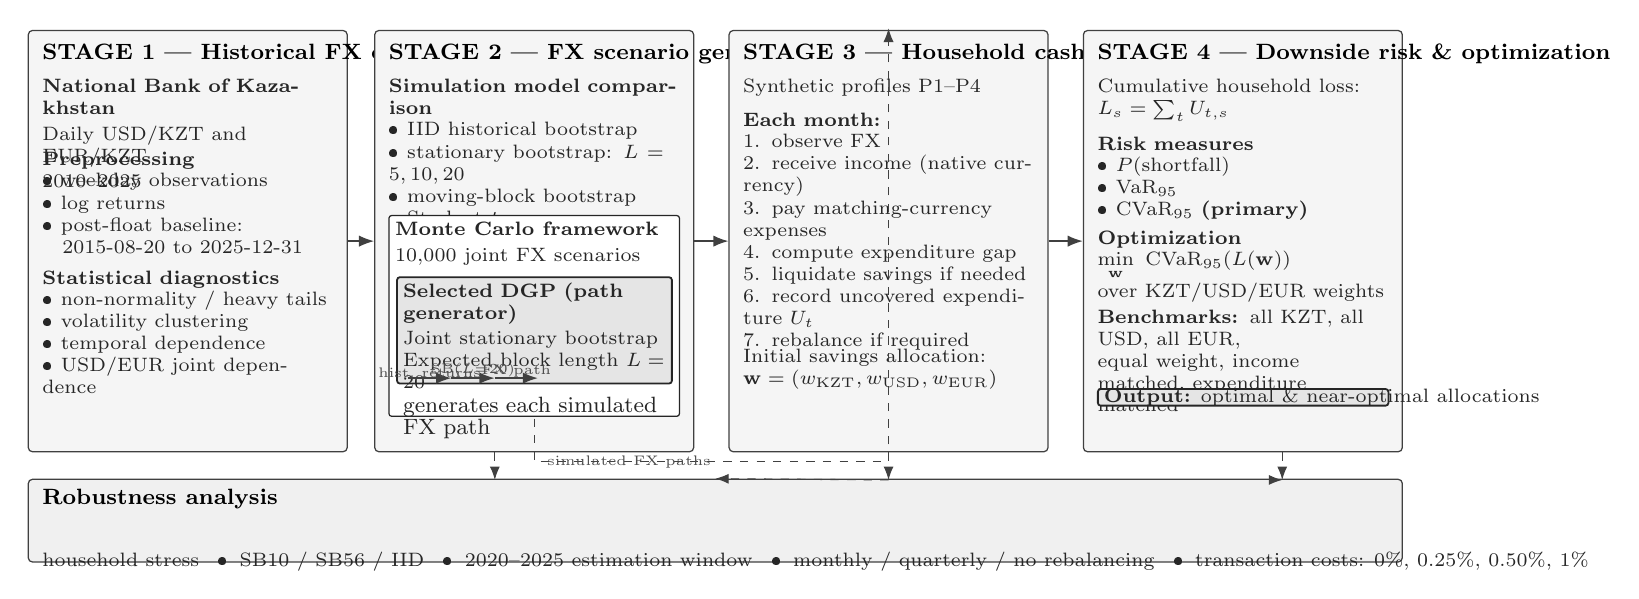
\begin{tikzpicture}[
  x=1cm, y=1cm,
  every node/.style={inner sep=0pt},
]

% --- layout constants (landscape ~17.5 x 8.5 cm) ---
\def\StageW{4.05}
\def\StageH{5.35}
\def\StageY{1.55}
\def\SOneX{0.15}
\def\STwoX{4.55}
\def\SThreeX{9.05}
\def\SFourX{13.55}
\def\RobustY{0.15}
\def\RobustH{1.05}

% ===================== STAGE 1 =====================
\node[stagebox, minimum width=\StageW cm, minimum height=\StageH cm, anchor=south west]
  (s1box) at (\SOneX,\StageY) {};
\node[stagetitle, anchor=north west] at ($(s1box.north west)+(0.18,-0.18)$)
  {STAGE 1 --- Historical FX data};
\node[bodytext, anchor=north west, text width=\StageW cm-0.36cm]
  at ($(s1box.north west)+(0.18,-0.62)$) {%
  \textbf{National Bank of Kazakhstan}\\[0.15em]
  Daily USD/KZT and EUR/KZT\\[0.15em]
  2010--2025
};
\node[bodytext, anchor=north west, text width=\StageW cm-0.36cm]
  at ($(s1box.north west)+(0.18,-1.55)$) {%
  \textbf{Preprocessing}\\[-0.05em]
  {\textbullet} weekday observations\\
  {\textbullet} log returns\\
  {\textbullet} post-float baseline:\\
  \hspace{0.9em}2015-08-20 to 2025-12-31
};
\node[bodytext, anchor=north west, text width=\StageW cm-0.36cm]
  at ($(s1box.north west)+(0.18,-3.05)$) {%
  \textbf{Statistical diagnostics}\\[-0.05em]
  {\textbullet} non-normality / heavy tails\\
  {\textbullet} volatility clustering\\
  {\textbullet} temporal dependence\\
  {\textbullet} USD/EUR joint dependence
};

% ===================== STAGE 2 =====================
\node[stagebox, minimum width=\StageW cm, minimum height=\StageH cm, anchor=south west]
  (s2box) at (\STwoX,\StageY) {};
\node[stagetitle, anchor=north west] at ($(s2box.north west)+(0.18,-0.18)$)
  {STAGE 2 --- FX scenario generation};

\node[bodytext, anchor=north west, text width=\StageW cm-0.36cm]
  at ($(s2box.north west)+(0.18,-0.62)$) {%
  \textbf{Simulation model comparison}\\[-0.05em]
  {\textbullet} IID historical bootstrap\\
  {\textbullet} stationary bootstrap: $L=5,10,20$\\
  {\textbullet} moving-block bootstrap\\
  {\textbullet} Student-$t$\\
  {\textbullet} Gaussian benchmark
};

% Monte Carlo outer frame
\node[nestedbox, minimum width=\StageW cm-0.36cm, minimum height=2.55cm,
  anchor=north west] (mcbox) at ($(s2box.north west)+(0.18,-2.35)$) {};
\node[bodytext, anchor=north west] at ($(mcbox.north west)+(0.08,-0.08)$)
  {\textbf{Monte Carlo framework}};
\node[bodytext, anchor=north west] at ($(mcbox.north west)+(0.08,-0.42)$)
  {10{,}000 joint FX scenarios};

% Selected DGP inside MC (explicit: SB generates each path)
\node[highlightbox, minimum width=\StageW cm-0.56cm, minimum height=1.35cm,
  anchor=north west] (dgpbox) at ($(mcbox.north west)+(0.10,-0.78)$) {};
\node[bodytext, anchor=north west, text width=\StageW cm-0.72cm]
  at ($(dgpbox.north west)+(0.08,-0.08)$) {%
  \textbf{Selected DGP (path generator)}\\[0.12em]
  Joint stationary bootstrap\\
  Expected block length $L=20$\\[0.08em]
  {\footnotesize generates each simulated FX path}
};

% Small schematic: historical returns -> SB -> path
\draw[flowarrow] ($(dgpbox.south west)+(0.15,0.08)$) -- ++(0.55,0)
  node[midway, above, font=\tiny, text=black!70] {hist.\ returns};
\draw[flowarrow] ($(dgpbox.south west)+(0.15,0.08)$) ++(0.55,0) -- ++(0.55,0)
  node[midway, above, font=\tiny, text=black!70] {SB($L{=}20$)};
\draw[flowarrow] ($(dgpbox.south west)+(0.15,0.08)$) ++(1.10,0) -- ++(0.55,0)
  node[midway, above, font=\tiny, text=black!70] {FX path};

% ===================== STAGE 3 =====================
\node[stagebox, minimum width=\StageW cm, minimum height=\StageH cm, anchor=south west]
  (s3box) at (\SThreeX,\StageY) {};
\node[stagetitle, anchor=north west] at ($(s3box.north west)+(0.18,-0.18)$)
  {STAGE 3 --- Household cash-flow simulation};

\node[bodytext, anchor=north west, text width=\StageW cm-0.36cm]
  at ($(s3box.north west)+(0.18,-0.62)$) {%
  Synthetic profiles P1--P4
};

\node[bodytext, anchor=north west, text width=\StageW cm-0.36cm]
  at ($(s3box.north west)+(0.18,-1.05)$) {%
  \textbf{Each month:}\\[-0.05em]
  {\scriptsize 1.} observe FX\\
  {\scriptsize 2.} receive income (native currency)\\
  {\scriptsize 3.} pay matching-currency expenses\\
  {\scriptsize 4.} compute expenditure gap\\
  {\scriptsize 5.} liquidate savings if needed\\
  {\scriptsize 6.} record uncovered expenditure $U_t$\\
  {\scriptsize 7.} rebalance if required
};

\node[bodytext, anchor=north west, text width=\StageW cm-0.36cm]
  at ($(s3box.north west)+(0.18,-4.05)$) {%
  Initial savings allocation:\\
  $\mathbf{w}=(w_{\mathrm{KZT}},w_{\mathrm{USD}},w_{\mathrm{EUR}})$
};

% ===================== STAGE 4 =====================
\node[stagebox, minimum width=\StageW cm, minimum height=\StageH cm, anchor=south west]
  (s4box) at (\SFourX,\StageY) {};
\node[stagetitle, anchor=north west] at ($(s4box.north west)+(0.18,-0.18)$)
  {STAGE 4 --- Downside risk \& optimization};

\node[bodytext, anchor=north west, text width=\StageW cm-0.36cm]
  at ($(s4box.north west)+(0.18,-0.62)$) {%
  Cumulative household loss:\\
  $L_s=\sum_t U_{t,s}$
};

\node[bodytext, anchor=north west, text width=\StageW cm-0.36cm]
  at ($(s4box.north west)+(0.18,-1.35)$) {%
  \textbf{Risk measures}\\[-0.05em]
  {\textbullet} $P(\text{shortfall})$\\
  {\textbullet} $\mathrm{VaR}_{95}$\\
  {\textbullet} $\mathrm{CVaR}_{95}$ \textbf{(primary)}
};

\node[bodytext, anchor=north west, text width=\StageW cm-0.36cm]
  at ($(s4box.north west)+(0.18,-2.55)$) {%
  \textbf{Optimization}\\[-0.05em]
  $\min\limits_{\mathbf{w}}\ \mathrm{CVaR}_{95}(L(\mathbf{w}))$\\
  over KZT/USD/EUR weights
};

\node[bodytext, anchor=north west, text width=\StageW cm-0.36cm]
  at ($(s4box.north west)+(0.18,-3.55)$) {%
  \textbf{Benchmarks:} all KZT, all USD, all EUR,\\
  equal weight, income matched, expenditure matched
};

\node[highlightbox, minimum width=\StageW cm-0.36cm, anchor=north west]
  (outbox) at ($(s4box.north west)+(0.18,-4.55)$) {};
\node[bodytext, anchor=west] at ($(outbox.west)+(0.08,0)$)
  {\textbf{Output:} optimal \& near-optimal allocations};

% ===================== MAIN FLOW ARROWS =====================
\draw[flowarrow] (s1box.east) -- (s2box.west);
\draw[flowarrow] (s2box.east) -- (s3box.west);
\draw[flowarrow] (s3box.east) -- (s4box.west);

% FX paths arrow from Stage 2 MC to Stage 3
\draw[flowarrow, dashed, line width=0.45pt]
  ($(mcbox.south)+(0,-0.02)$) -- ++(0,-0.55)
  -| ($(s3box.north)+(0,0.02)$)
  node[pos=0.25, font=\tiny, text=black!70, left] {simulated FX paths};

% ===================== ROBUSTNESS STRIP =====================
\node[robustbox, minimum width=17.45cm, minimum height=\RobustH cm, anchor=south west]
  (rbox) at (0.15,\RobustY) {};
\node[stagetitle, anchor=north west] at ($(rbox.north west)+(0.18,-0.12)$)
  {Robustness analysis};
\node[bodytext, anchor=west] at ($(rbox.west)+(0.18,-0.52)$) {%
  household stress \enspace\textbullet\enspace
  SB10 / SB56 / IID \enspace\textbullet\enspace
  2020--2025 estimation window \enspace\textbullet\enspace
  monthly / quarterly / no rebalancing \enspace\textbullet\enspace
  transaction costs: 0\%, 0.25\%, 0.50\%, 1\%
};

% Connect robustness to pipeline (Stages 2--4)
\draw[flowarrow, line width=0.4pt, dashed]
  ($(s2box.south)+(-0.5,0)$) -- ++(0,-0.35);
\draw[flowarrow, line width=0.4pt, dashed]
  ($(s3box.south)+(0,0)$) -- ++(0,-0.35);
\draw[flowarrow, line width=0.4pt, dashed]
  ($(s4box.south)+(0.5,0)$) -- ++(0,-0.35);
\draw[flowarrow, line width=0.4pt, dashed]
  ($(s2box.south)+(-0.5,-0.35)$) -- ($(s4box.south)+(0.5,-0.35)$);
\draw[flowarrow, line width=0.4pt, dashed]
  ($(s3box.south)+(0,-0.35)$) -- ($(rbox.north)+(0,0)$);

\end{tikzpicture}


\documentclass[tikz,border=0pt]{standalone}

\usepackage[T1]{fontenc}
\usepackage{lmodern}
\usepackage{amsmath,amssymb}
\usepackage{tikz}
\usetikzlibrary{
  arrows.meta,
  positioning,
  calc,
  fit,
  backgrounds,
}

% Journal-style palette (grayscale-safe)
\colorlet{StageFill}{black!4}
\colorlet{StageLine}{black!75}
\colorlet{AccentFill}{black!10}
\colorlet{AccentLine}{black!85}
\colorlet{RobustFill}{black!6}

\tikzset{
  >=Latex,
  stagebox/.style={
    draw=StageLine,
    line width=0.45pt,
    fill=StageFill,
    rounded corners=1.5pt,
    inner sep=0pt,
  },
  stagetitle/.style={
    font=\footnotesize\bfseries,
    text=black,
  },
  bodytext/.style={
    font=\scriptsize,
    text=black!85,
    align=left,
  },
  bullet/.style={
    font=\scriptsize,
    text=black!85,
    align=left,
  },
  flowarrow/.style={
    ->,
    line width=0.55pt,
    draw=StageLine,
  },
  nestedbox/.style={
    draw=AccentLine,
    line width=0.45pt,
    fill=white,
    rounded corners=1pt,
    inner sep=3pt,
  },
  highlightbox/.style={
    draw=AccentLine,
    line width=0.65pt,
    fill=AccentFill,
    rounded corners=1pt,
    inner sep=3pt,
  },
  robustbox/.style={
    draw=StageLine,
    line width=0.45pt,
    fill=RobustFill,
    rounded corners=1.5pt,
    inner sep=4pt,
  },
}

\begin{document}
% research_framework.tikz — publication framework figure (fig:research_framework)
% Landscape; intended for figure* in two-column layout.

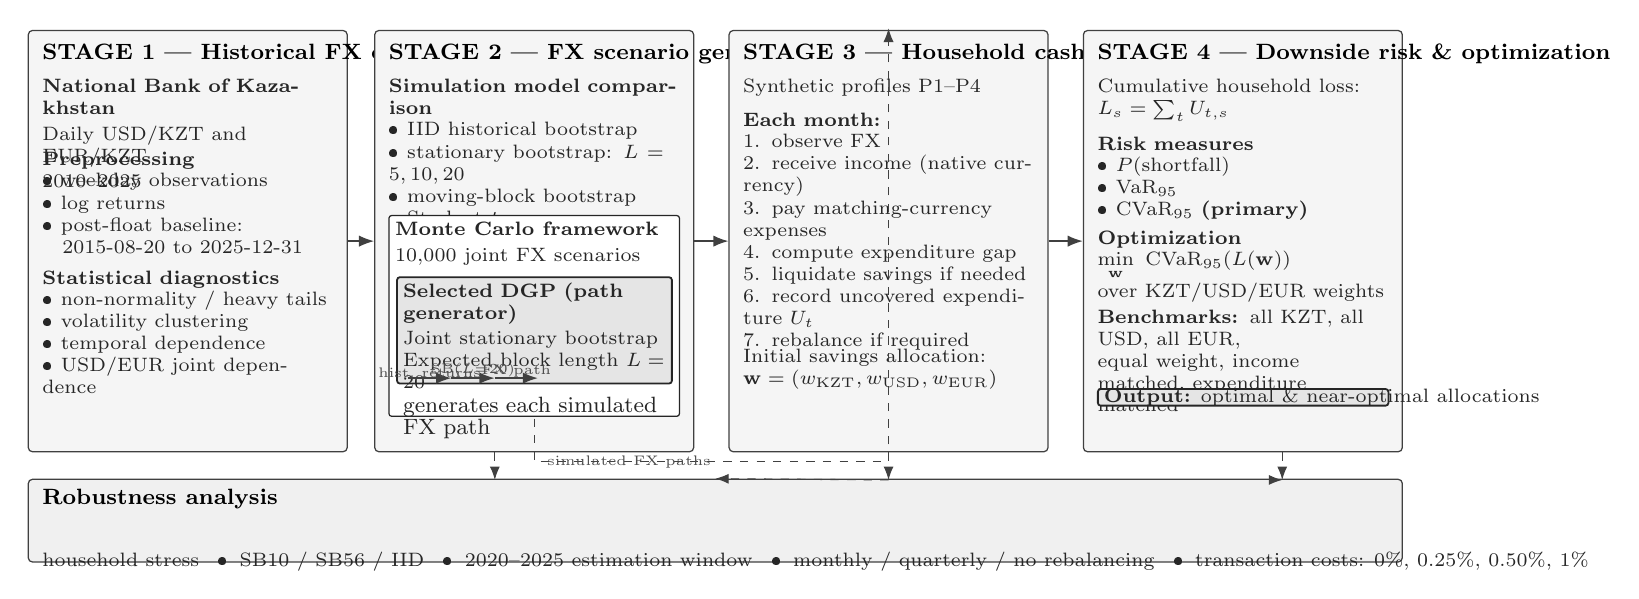
\begin{tikzpicture}[
  x=1cm, y=1cm,
  every node/.style={inner sep=0pt},
]

% --- layout constants (landscape ~17.5 x 8.5 cm) ---
\def\StageW{4.05}
\def\StageH{5.35}
\def\StageY{1.55}
\def\SOneX{0.15}
\def\STwoX{4.55}
\def\SThreeX{9.05}
\def\SFourX{13.55}
\def\RobustY{0.15}
\def\RobustH{1.05}

% ===================== STAGE 1 =====================
\node[stagebox, minimum width=\StageW cm, minimum height=\StageH cm, anchor=south west]
  (s1box) at (\SOneX,\StageY) {};
\node[stagetitle, anchor=north west] at ($(s1box.north west)+(0.18,-0.18)$)
  {STAGE 1 --- Historical FX data};
\node[bodytext, anchor=north west, text width=\StageW cm-0.36cm]
  at ($(s1box.north west)+(0.18,-0.62)$) {%
  \textbf{National Bank of Kazakhstan}\\[0.15em]
  Daily USD/KZT and EUR/KZT\\[0.15em]
  2010--2025
};
\node[bodytext, anchor=north west, text width=\StageW cm-0.36cm]
  at ($(s1box.north west)+(0.18,-1.55)$) {%
  \textbf{Preprocessing}\\[-0.05em]
  {\textbullet} weekday observations\\
  {\textbullet} log returns\\
  {\textbullet} post-float baseline:\\
  \hspace{0.9em}2015-08-20 to 2025-12-31
};
\node[bodytext, anchor=north west, text width=\StageW cm-0.36cm]
  at ($(s1box.north west)+(0.18,-3.05)$) {%
  \textbf{Statistical diagnostics}\\[-0.05em]
  {\textbullet} non-normality / heavy tails\\
  {\textbullet} volatility clustering\\
  {\textbullet} temporal dependence\\
  {\textbullet} USD/EUR joint dependence
};

% ===================== STAGE 2 =====================
\node[stagebox, minimum width=\StageW cm, minimum height=\StageH cm, anchor=south west]
  (s2box) at (\STwoX,\StageY) {};
\node[stagetitle, anchor=north west] at ($(s2box.north west)+(0.18,-0.18)$)
  {STAGE 2 --- FX scenario generation};

\node[bodytext, anchor=north west, text width=\StageW cm-0.36cm]
  at ($(s2box.north west)+(0.18,-0.62)$) {%
  \textbf{Simulation model comparison}\\[-0.05em]
  {\textbullet} IID historical bootstrap\\
  {\textbullet} stationary bootstrap: $L=5,10,20$\\
  {\textbullet} moving-block bootstrap\\
  {\textbullet} Student-$t$\\
  {\textbullet} Gaussian benchmark
};

% Monte Carlo outer frame
\node[nestedbox, minimum width=\StageW cm-0.36cm, minimum height=2.55cm,
  anchor=north west] (mcbox) at ($(s2box.north west)+(0.18,-2.35)$) {};
\node[bodytext, anchor=north west] at ($(mcbox.north west)+(0.08,-0.08)$)
  {\textbf{Monte Carlo framework}};
\node[bodytext, anchor=north west] at ($(mcbox.north west)+(0.08,-0.42)$)
  {10{,}000 joint FX scenarios};

% Selected DGP inside MC (explicit: SB generates each path)
\node[highlightbox, minimum width=\StageW cm-0.56cm, minimum height=1.35cm,
  anchor=north west] (dgpbox) at ($(mcbox.north west)+(0.10,-0.78)$) {};
\node[bodytext, anchor=north west, text width=\StageW cm-0.72cm]
  at ($(dgpbox.north west)+(0.08,-0.08)$) {%
  \textbf{Selected DGP (path generator)}\\[0.12em]
  Joint stationary bootstrap\\
  Expected block length $L=20$\\[0.08em]
  {\footnotesize generates each simulated FX path}
};

% Small schematic: historical returns -> SB -> path
\draw[flowarrow] ($(dgpbox.south west)+(0.15,0.08)$) -- ++(0.55,0)
  node[midway, above, font=\tiny, text=black!70] {hist.\ returns};
\draw[flowarrow] ($(dgpbox.south west)+(0.15,0.08)$) ++(0.55,0) -- ++(0.55,0)
  node[midway, above, font=\tiny, text=black!70] {SB($L{=}20$)};
\draw[flowarrow] ($(dgpbox.south west)+(0.15,0.08)$) ++(1.10,0) -- ++(0.55,0)
  node[midway, above, font=\tiny, text=black!70] {FX path};

% ===================== STAGE 3 =====================
\node[stagebox, minimum width=\StageW cm, minimum height=\StageH cm, anchor=south west]
  (s3box) at (\SThreeX,\StageY) {};
\node[stagetitle, anchor=north west] at ($(s3box.north west)+(0.18,-0.18)$)
  {STAGE 3 --- Household cash-flow simulation};

\node[bodytext, anchor=north west, text width=\StageW cm-0.36cm]
  at ($(s3box.north west)+(0.18,-0.62)$) {%
  Synthetic profiles P1--P4
};

\node[bodytext, anchor=north west, text width=\StageW cm-0.36cm]
  at ($(s3box.north west)+(0.18,-1.05)$) {%
  \textbf{Each month:}\\[-0.05em]
  {\scriptsize 1.} observe FX\\
  {\scriptsize 2.} receive income (native currency)\\
  {\scriptsize 3.} pay matching-currency expenses\\
  {\scriptsize 4.} compute expenditure gap\\
  {\scriptsize 5.} liquidate savings if needed\\
  {\scriptsize 6.} record uncovered expenditure $U_t$\\
  {\scriptsize 7.} rebalance if required
};

\node[bodytext, anchor=north west, text width=\StageW cm-0.36cm]
  at ($(s3box.north west)+(0.18,-4.05)$) {%
  Initial savings allocation:\\
  $\mathbf{w}=(w_{\mathrm{KZT}},w_{\mathrm{USD}},w_{\mathrm{EUR}})$
};

% ===================== STAGE 4 =====================
\node[stagebox, minimum width=\StageW cm, minimum height=\StageH cm, anchor=south west]
  (s4box) at (\SFourX,\StageY) {};
\node[stagetitle, anchor=north west] at ($(s4box.north west)+(0.18,-0.18)$)
  {STAGE 4 --- Downside risk \& optimization};

\node[bodytext, anchor=north west, text width=\StageW cm-0.36cm]
  at ($(s4box.north west)+(0.18,-0.62)$) {%
  Cumulative household loss:\\
  $L_s=\sum_t U_{t,s}$
};

\node[bodytext, anchor=north west, text width=\StageW cm-0.36cm]
  at ($(s4box.north west)+(0.18,-1.35)$) {%
  \textbf{Risk measures}\\[-0.05em]
  {\textbullet} $P(\text{shortfall})$\\
  {\textbullet} $\mathrm{VaR}_{95}$\\
  {\textbullet} $\mathrm{CVaR}_{95}$ \textbf{(primary)}
};

\node[bodytext, anchor=north west, text width=\StageW cm-0.36cm]
  at ($(s4box.north west)+(0.18,-2.55)$) {%
  \textbf{Optimization}\\[-0.05em]
  $\min\limits_{\mathbf{w}}\ \mathrm{CVaR}_{95}(L(\mathbf{w}))$\\
  over KZT/USD/EUR weights
};

\node[bodytext, anchor=north west, text width=\StageW cm-0.36cm]
  at ($(s4box.north west)+(0.18,-3.55)$) {%
  \textbf{Benchmarks:} all KZT, all USD, all EUR,\\
  equal weight, income matched, expenditure matched
};

\node[highlightbox, minimum width=\StageW cm-0.36cm, anchor=north west]
  (outbox) at ($(s4box.north west)+(0.18,-4.55)$) {};
\node[bodytext, anchor=west] at ($(outbox.west)+(0.08,0)$)
  {\textbf{Output:} optimal \& near-optimal allocations};

% ===================== MAIN FLOW ARROWS =====================
\draw[flowarrow] (s1box.east) -- (s2box.west);
\draw[flowarrow] (s2box.east) -- (s3box.west);
\draw[flowarrow] (s3box.east) -- (s4box.west);

% FX paths arrow from Stage 2 MC to Stage 3
\draw[flowarrow, dashed, line width=0.45pt]
  ($(mcbox.south)+(0,-0.02)$) -- ++(0,-0.55)
  -| ($(s3box.north)+(0,0.02)$)
  node[pos=0.25, font=\tiny, text=black!70, left] {simulated FX paths};

% ===================== ROBUSTNESS STRIP =====================
\node[robustbox, minimum width=17.45cm, minimum height=\RobustH cm, anchor=south west]
  (rbox) at (0.15,\RobustY) {};
\node[stagetitle, anchor=north west] at ($(rbox.north west)+(0.18,-0.12)$)
  {Robustness analysis};
\node[bodytext, anchor=west] at ($(rbox.west)+(0.18,-0.52)$) {%
  household stress \enspace\textbullet\enspace
  SB10 / SB56 / IID \enspace\textbullet\enspace
  2020--2025 estimation window \enspace\textbullet\enspace
  monthly / quarterly / no rebalancing \enspace\textbullet\enspace
  transaction costs: 0\%, 0.25\%, 0.50\%, 1\%
};

% Connect robustness to pipeline (Stages 2--4)
\draw[flowarrow, line width=0.4pt, dashed]
  ($(s2box.south)+(-0.5,0)$) -- ++(0,-0.35);
\draw[flowarrow, line width=0.4pt, dashed]
  ($(s3box.south)+(0,0)$) -- ++(0,-0.35);
\draw[flowarrow, line width=0.4pt, dashed]
  ($(s4box.south)+(0.5,0)$) -- ++(0,-0.35);
\draw[flowarrow, line width=0.4pt, dashed]
  ($(s2box.south)+(-0.5,-0.35)$) -- ($(s4box.south)+(0.5,-0.35)$);
\draw[flowarrow, line width=0.4pt, dashed]
  ($(s3box.south)+(0,-0.35)$) -- ($(rbox.north)+(0,0)$);

\end{tikzpicture}

\end{document}
